\documentclass[aspectratio=169]{beamer}
\usepackage[utf8]{inputenc}
\usepackage{hyperref}
\usepackage{amsmath,amsfonts,amsthm,bm}
\usepackage{color}
\usepackage{minted}
\usepackage{graphicx} % Allows including images
\usepackage{booktabs} % Allows the use of \toprule, \midrule and \bottomrule in tables
\usepackage{tikz}
\usepackage[version=3]{mhchem}
\usepackage{pgfplots}
\pgfplotsset{compat=1.16} 
\setminted{fontsize=\scriptsize}
\usepackage{multirow}

\hypersetup{
    colorlinks=true,
    linkcolor=red,
    filecolor=magenta,      
    urlcolor=red,
}

\DeclareMathOperator*{\argmax}{argmax}
\DeclareMathOperator*{\argmin}{argmin}
\let \vec \mathbf

\mode<presentation> {
    \usetheme{CambridgeUS}
    %\setbeamertemplate{footline} % To remove the footer line in all slides uncomment this line
    \setbeamertemplate{footline}[page number] % To replace the footer line in all slides with a simple slide count uncomment this line
    \setbeamertemplate{navigation symbols}{} % To remove the navigation symbols from the bottom of all slides uncomment this line
}


\title[NANO281 Review]{NANO281 Review}

\author{Shyue Ping Ong}
\institute[UCSD]{University of California, San Diego\\
\medskip
}
\date{NANO281} % Date, can be changed to a custom date

\begin{document}


\begin{frame}
    \titlepage % Print the title page as the first slide
\end{frame}


\begin{frame}{Overview}
    \tableofcontents
\end{frame}


\section{Review}


\begin{frame}{Preliminaries}
    \begin{itemize}
        \item In this class, we have provided a broad survey of data science techniques as they are applied to materials science problems.
        \item In doing so, we have opted for breadth rather than depth, and eschewed most of the mathematical derivations that is typical in data science classes.
        \item In this final lecture, I want to do an overview of the coverage to reinforce the lessons learnt.
        \item The structure of this overview is deliberately different from the sequence in which we have done the entire class. Now that you have the details in your mind, this lecture provides a high-level overview of key takeaways and guiding principles.
    \end{itemize}
\end{frame}


\begin{frame}{Why Data Science?}
    \begin{itemize}
        \item Materials data is exploding in quantity and quality.
        \begin{itemize}
            \item High-throughput/combinatorial experiments.
            \item High-throughput first principles computations.
        \end{itemize}
        \item Types of problems that can most benefit from data science:
        \begin{itemize}
            \item Things that are still too difficult to perform experiments on or compute.
            \item Relationships that are beyond our understanding (at the present moment). 
        \end{itemize}
    \end{itemize}
\end{frame}


\begin{frame}{ML flowchart}
\begin{figure}
    \centering
    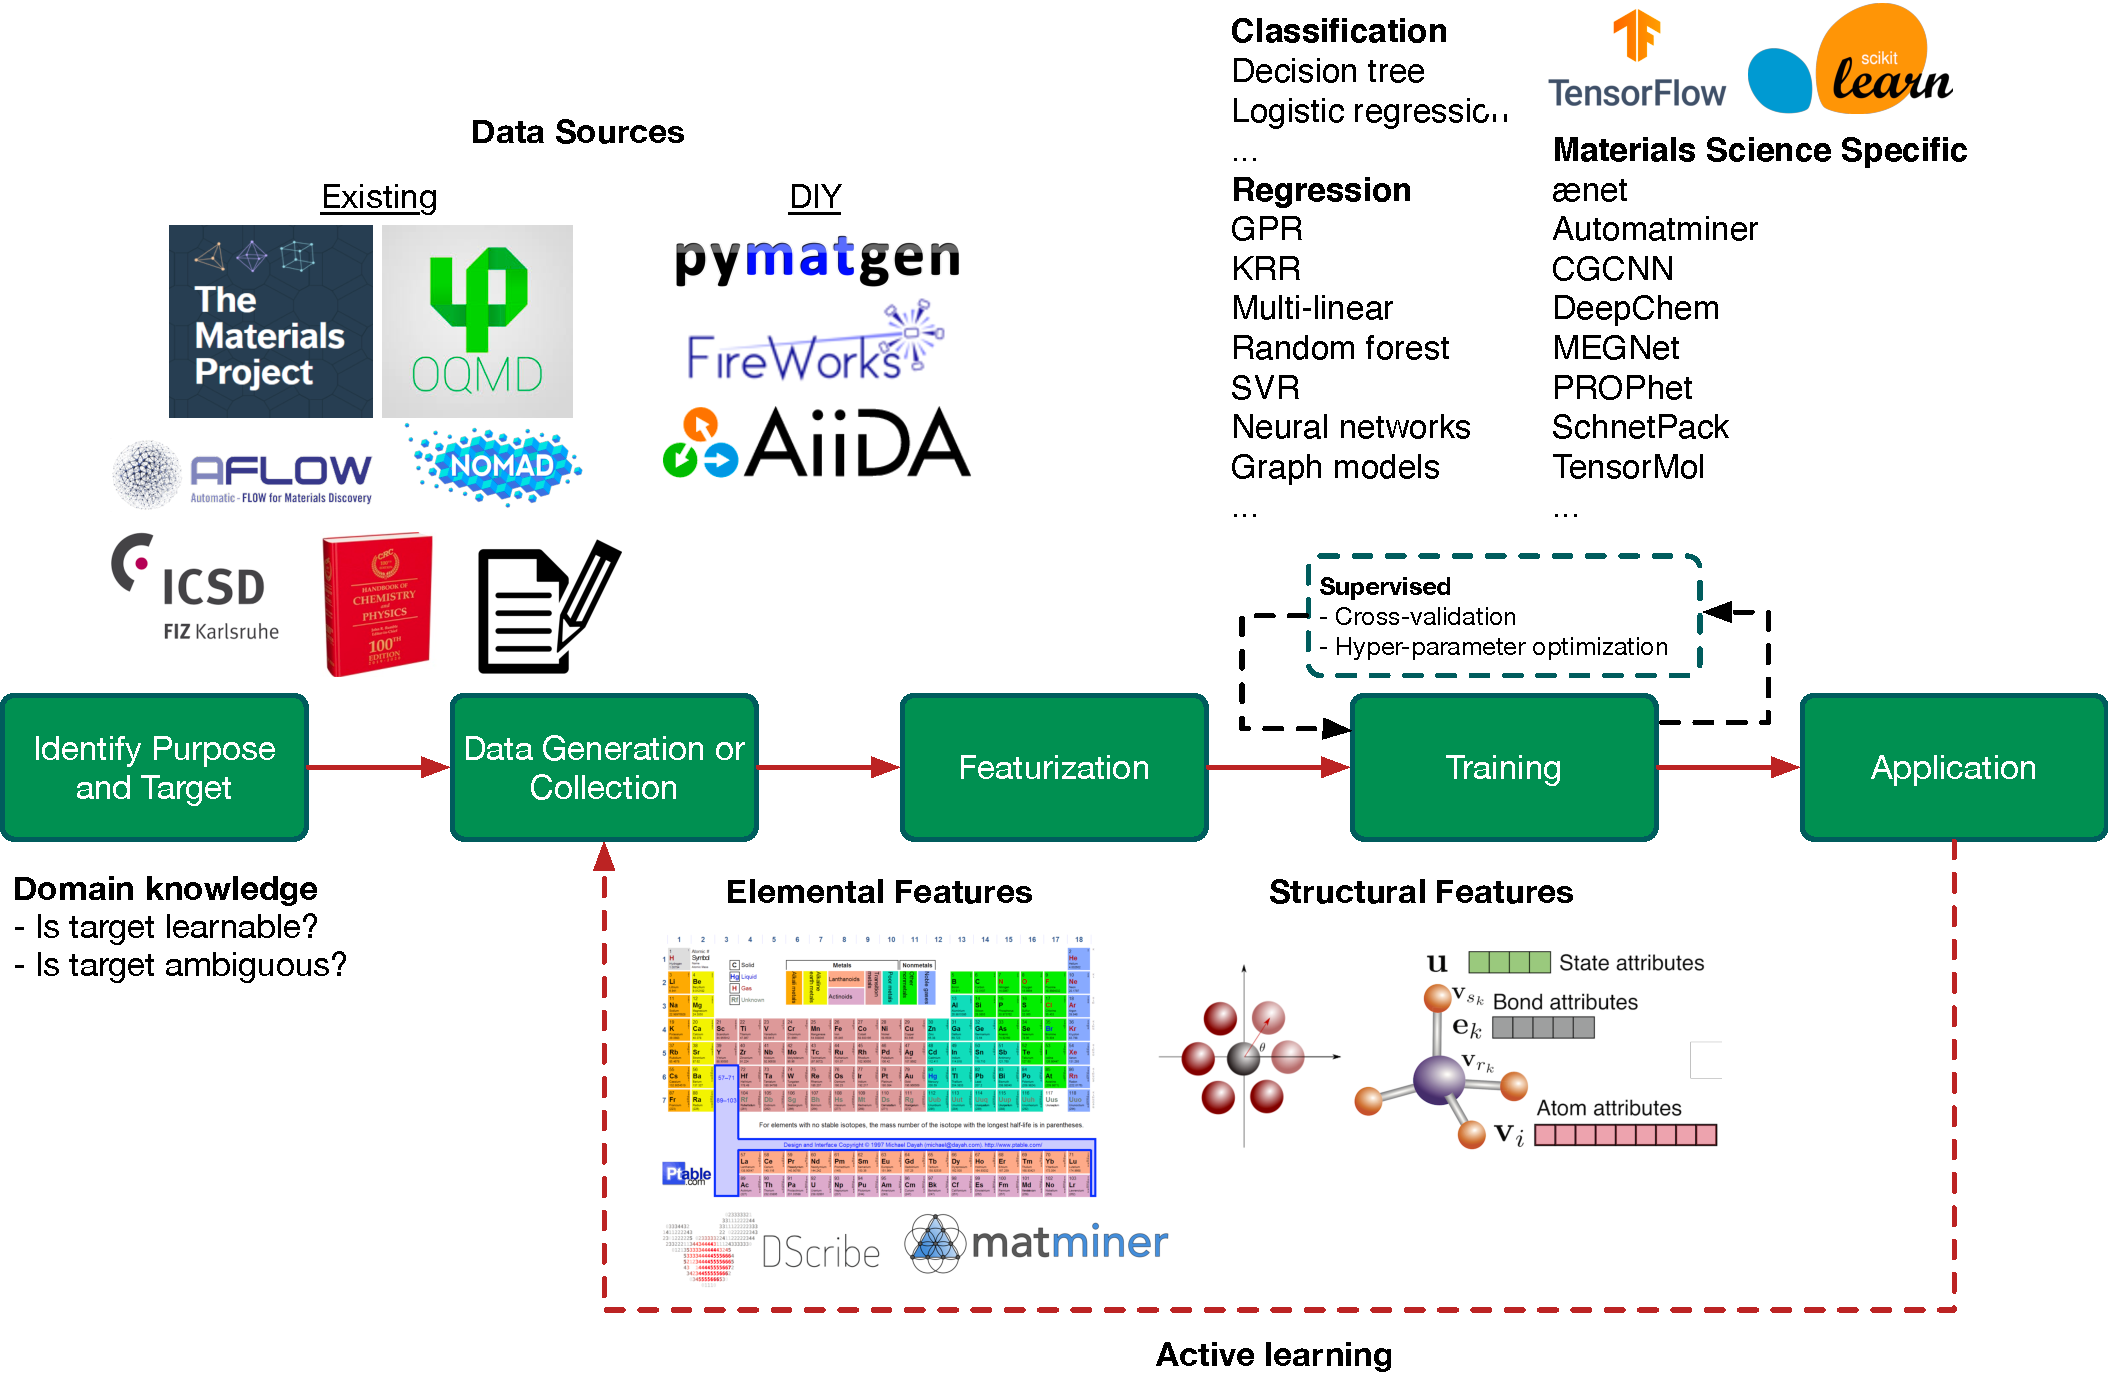
\includegraphics[width=0.65\textwidth]{figures/ml_flowchart.pdf}
\end{figure}
\end{frame}


\begin{frame}{Data and Featurization}
    \begin{itemize}
        \item Data generation, collection and wrangling is typically the most time-consuming portion of the whole process.
        \item Sources: Experimental (\href{http://icsd.fiz-karlsruhe.de/icsd/}{ICSD}, \href{http://paulingfile.com/}{Pauling file}, literature, ...), Computational (\href{http://www.materialsproject.org}{Materials Project}, \href{http://oqmd.org/}{OQMD}, \href{http://aflowlib.org/}{AFLOW}, \href{https://nomad-coe.eu/}{NOMAD}, ...).
        \item Quality and quantity remains a big issue in materials science.
        \item Featurization - typically the choice that affects model performance the most
        \begin{itemize}
            \item Composition-based features (e.g., electronegativity, atomic radii, etc.): intuitively simple, readily available, but clearly cannot capture structural differences.
            \item Structure-based features (including graphs): much greater complexity, typically must obey symmetries of system to be effective.
        \end{itemize}
    \end{itemize}
\end{frame}


\begin{frame}{Model fitting}
    \begin{itemize}
        \item All model fittings follow the same basic principle - minimizing of some \textit{loss function}, $L(\theta; y_i, \vec{x_i})$ either analytically or by numerical procedures (e.g., gradient descent).
    \end{itemize}
        \begin{table}[h]
        \scriptsize
            \centering
            \begin{tabular}{l|l|l}
                Task & Loss function & Equation \\
                \hline
             \multirow{2}{*}{Regression} & Mean squared error & $
        \sum_{i=1}^N (y_i - f(x_i))^2$\\
        & Mean absolute error & $
        \sum_{i=1}^N |y_i - f(x_i)|$\\
               \hline \multirow{4}{*}{Classification} & Missclassification rate & $I(\mathrm{sign}(f) \neq y)$\\
               & Exponential loss & $e^{-yf(x)}$\\
                 & Binomial/multinomial &
        $-\sum_{k=1}^K I(y=G_k)f_k(x) + \log \left(\sum_{l=1}^K e^{f_l(x)}\right)$\\
        & Binomial deviance & $\log(1 + e^{-2yf})$
            \end{tabular}
        \end{table}
\end{frame}


\begin{frame}{Model assessment and selection}
    \begin{itemize}
        \item Model performance is related to its performance on \textit{independent test data}.
        \begin{itemize}
            \item Training error: $L$ over training set.
            \item Test error: $L$ over independent test set.
        \end{itemize}
        \item Model complexity increases as the number of parameters increases. 
        \item Training errors \textbf{always} decrease with increasing model complexity.
        \item Test errors are high when model complexity is too low (underfitting) or too high (overfitting).
    \end{itemize}
    \begin{figure}
        \centering
        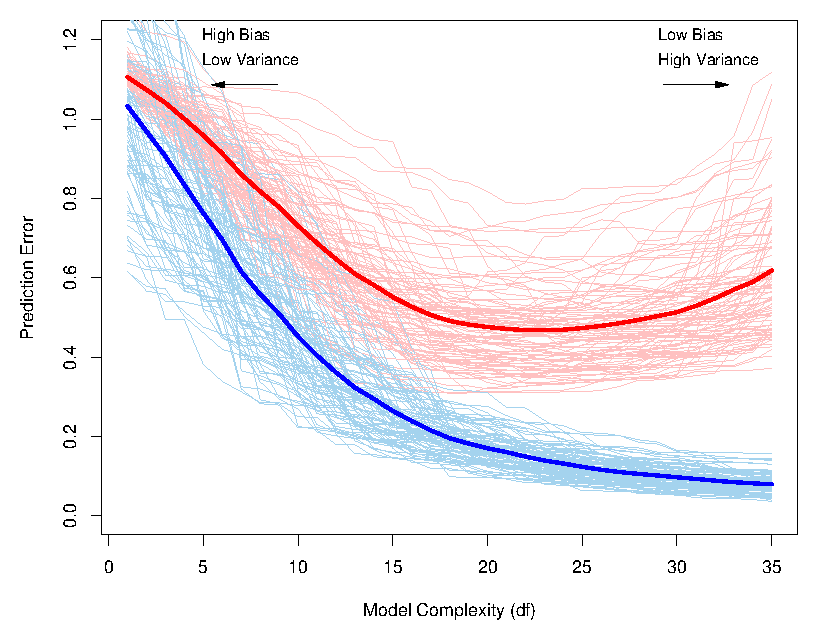
\includegraphics[width=0.25\textwidth]{figures/fig7-1.pdf}
    \end{figure}
\end{frame} 


\begin{frame}{Training, validation and test data}
    \begin{itemize}
        \item Model selection: estimating the performance of different models in order to choose the best one.
        \item Model assessment: having chosen a final model, estimating its prediction error (generalization error) on new data.
        \begin{itemize}
            \item Training set: For training the model.
            \item Validation set: For estimating prediction error to select the model.
            \item Test set: For assessing the generalization error of the final model. This should not be used in fitting the model.
        \end{itemize}
        \item Typical training:validation:test split is 50:25:25 or 80:10:10, or in very data-poor situations, maybe even 90:5:5.
    \end{itemize}
\end{frame}


\begin{frame}{$K$-fold cross validation (CV)}
    \begin{itemize}
        \item Simplest and most widely used approach for model validation.
        \item Data set is split into $K$ buckets (usually by random).
        \item Typical values of $K$ is 5 or 10. $K = N$ is known as ``leave-one-out'' CV.
        \begin{table}
        \begin{tabular}{|p{1.7cm}|p{1.7cm}|p{1.7cm}|p{1.7cm}|p{1.7cm}|}
            \hline
            \Large{Train} & \Large{Train} & \textcolor{red}{\Large{Validate}} & \Large{Train} & \Large{Train}\\
            \hline
        \end{tabular}
        \end{table}
        \item CV score is computed on the validate data set after training on the train data:
        \begin{equation*}
                CV(\hat{f}^{-k(i)},\alpha) = \frac{1}{N_{k(i)}}\sum_{i=1}^{N_{k(i)}} L(y_i, \hat{f}^{-k(i)}(x_i,\alpha))
        \end{equation*}
        \item assuming the $k^{th}$ data bucket has $N_{k(i)}$ data points and $\hat{f}^{-k(i)}$ refers to the model fitted with the $k^{th}$ data left out.
    \end{itemize}
\end{frame}


\begin{frame}{Regularization}
    \begin{itemize}
        \item Often, one starts from a model that is more complex first, and then reduce model complexity.
        \item Reducing model complexity decreases risk of overfitting (improve generalizability).
        \begin{itemize}
            \item Shrink coefficients or weights, sometimes to zero.
            \item Subset selection / tree pruning.
        \end{itemize}
        \item General approach is to add a \textit{penalty term} to loss functions that penalizes overcomplex models, e.g., sum of squares or absolute value of coefficients (e.g., MLR) or weights (NNs), tree size (decision trees), etc. Controlled by some parameter to be specified by model developer that determines size of penalty.
        \item Bias-variance trade-off:
        \begin{equation*}
            \mathrm{MSE} = \mathrm{var}(\hat{\theta}) + [E(\hat{\theta}) - \theta]^2
        \end{equation*}
    \end{itemize}
\end{frame}


\begin{frame}{Types of ML models}
    \begin{itemize}
        \item Supervised learning
        \begin{itemize}
            \item Linear (MLR, Ridge, Lasso, Linear/Quadratic Discriminant)
            \item Local/Kernel methods (kNN, kernel density estimation, Gaussian mixture models)
            \item Trees (CART, Adaboost, Gradient Boosting, Random Forest)
            \item Neural networks
        \end{itemize}
        \item Unsupervised learning
        \begin{itemize}
            \item Principal Component Analysis
            \item K-means
            \item Hierarchical clustering
            \item DBSCAN
        \end{itemize}
        \item Most models can be made more flexible through basis expansions (polynomial, Gaussian, cubic splines, etc.)
        \item Many other models have not been covered (e.g., support vector machines, graph-based models, etc.)
    \end{itemize}
\end{frame}


\section{Final Lab}

\begin{frame}{Final Lab}
    \begin{itemize}
        \item Working on an \textbf{open} problem in materials science.
        \item Will be held as a Kaggle competition - see Canvas for link.
        \item If the results are sufficiently good, the whole class will write a journal article on the results.
        \item Top three results within 10\% in accuracy of each other will be co-first authors. All students will be co-authors.
        \item Note that the actual results have no impact on grades - for grading purposes, we are looking at proper application of data science techniques for the problem, not raw accuracy. Of course, if the accuracy is far lower than what others have obtained, it typically means you are not doing something correctly.
    \end{itemize}
\end{frame}


 \begin{frame}{X-ray diffraction}
 \begin{figure}
     \centering
     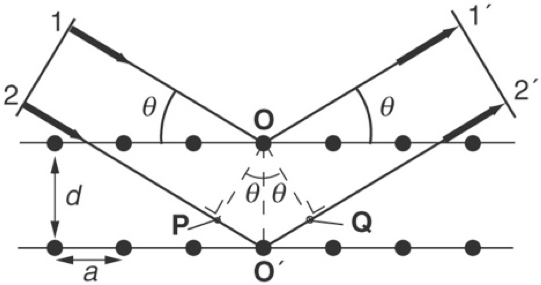
\includegraphics[width=0.5\textwidth]{figures/xrd.png}
 \end{figure}
    \begin{itemize}
        \item X-ray diffraction (XRD) is a technique for determining the structure of crystals and is frequently used for phase identification. Planes in a crystal cause a beam of incident X-rays to diffract into many specific directions.
    \end{itemize}
\end{frame}


\begin{frame}{XRD pattern}
\begin{figure}
    \centering
    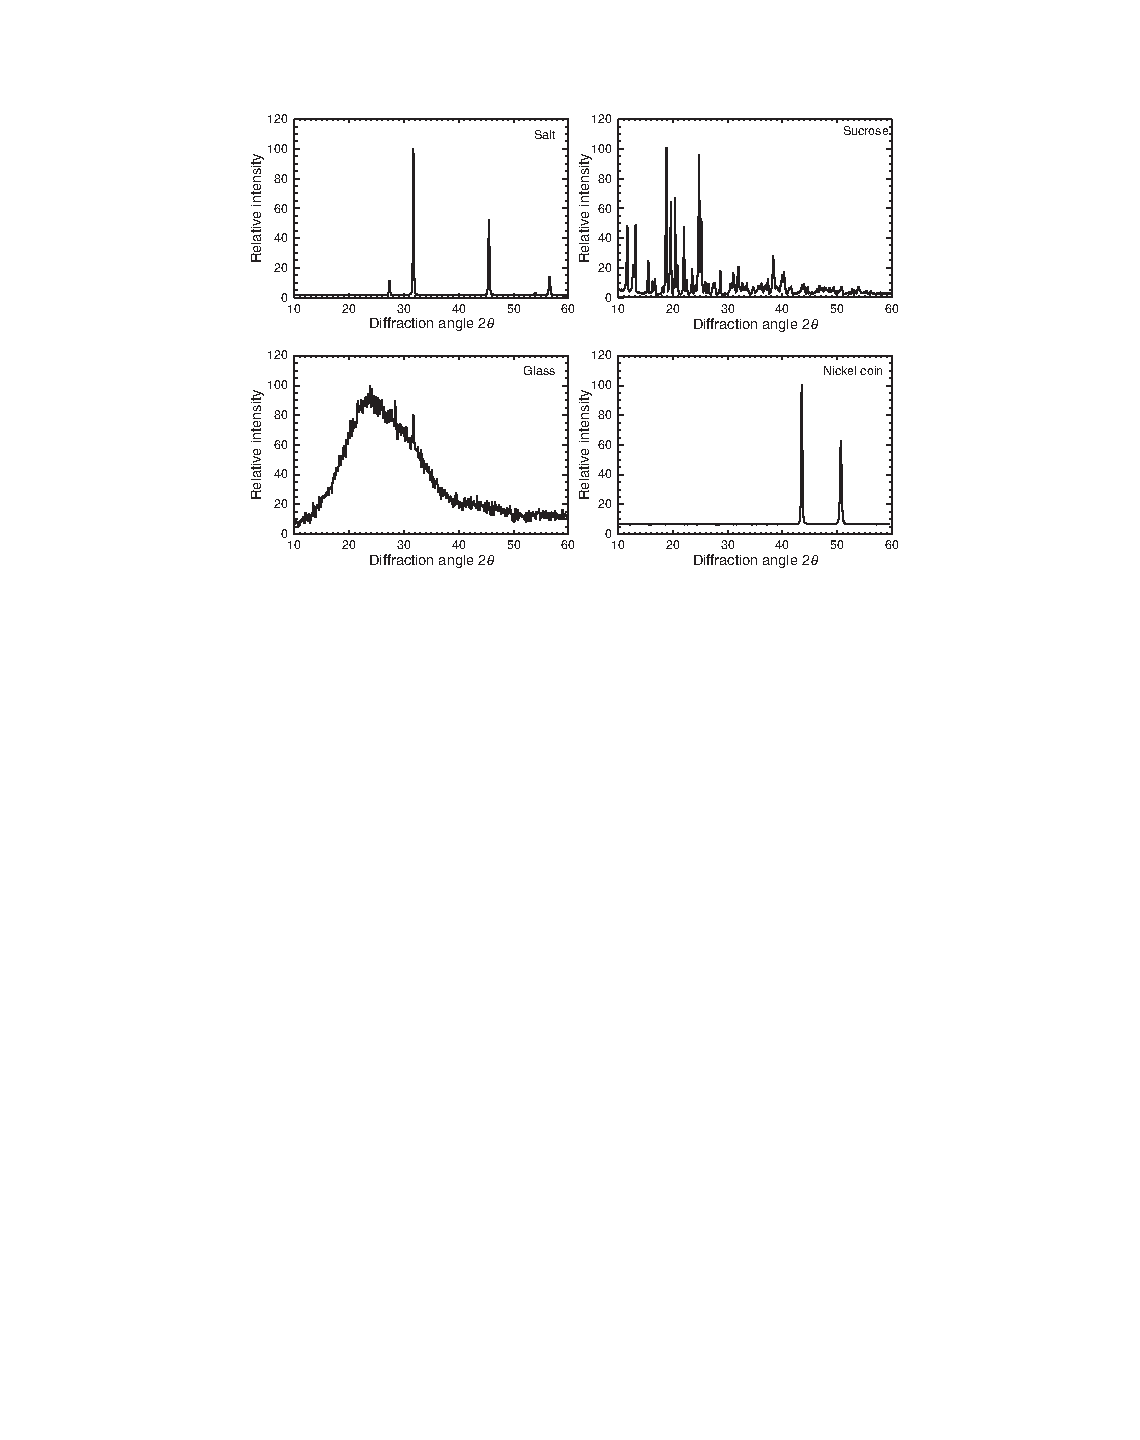
\includegraphics[width=0.4\textwidth]{figures/xrd_patterns.pdf}
\end{figure}
\begin{itemize}
    \item Peak positions (given in $2\theta$) are given by Bragg's equation: $2d \sin{\theta} = \lambda$, where $\lambda$ is the wavelength of the X-ray and $d$ is the interplanar spacing.
    \item Peak intensities are given the nature of the atomic species and the presence of various symmetries (e.g., centering atoms).
\end{itemize}
\end{frame}


\begin{frame}{The challenge}
\begin{figure}
    \centering
    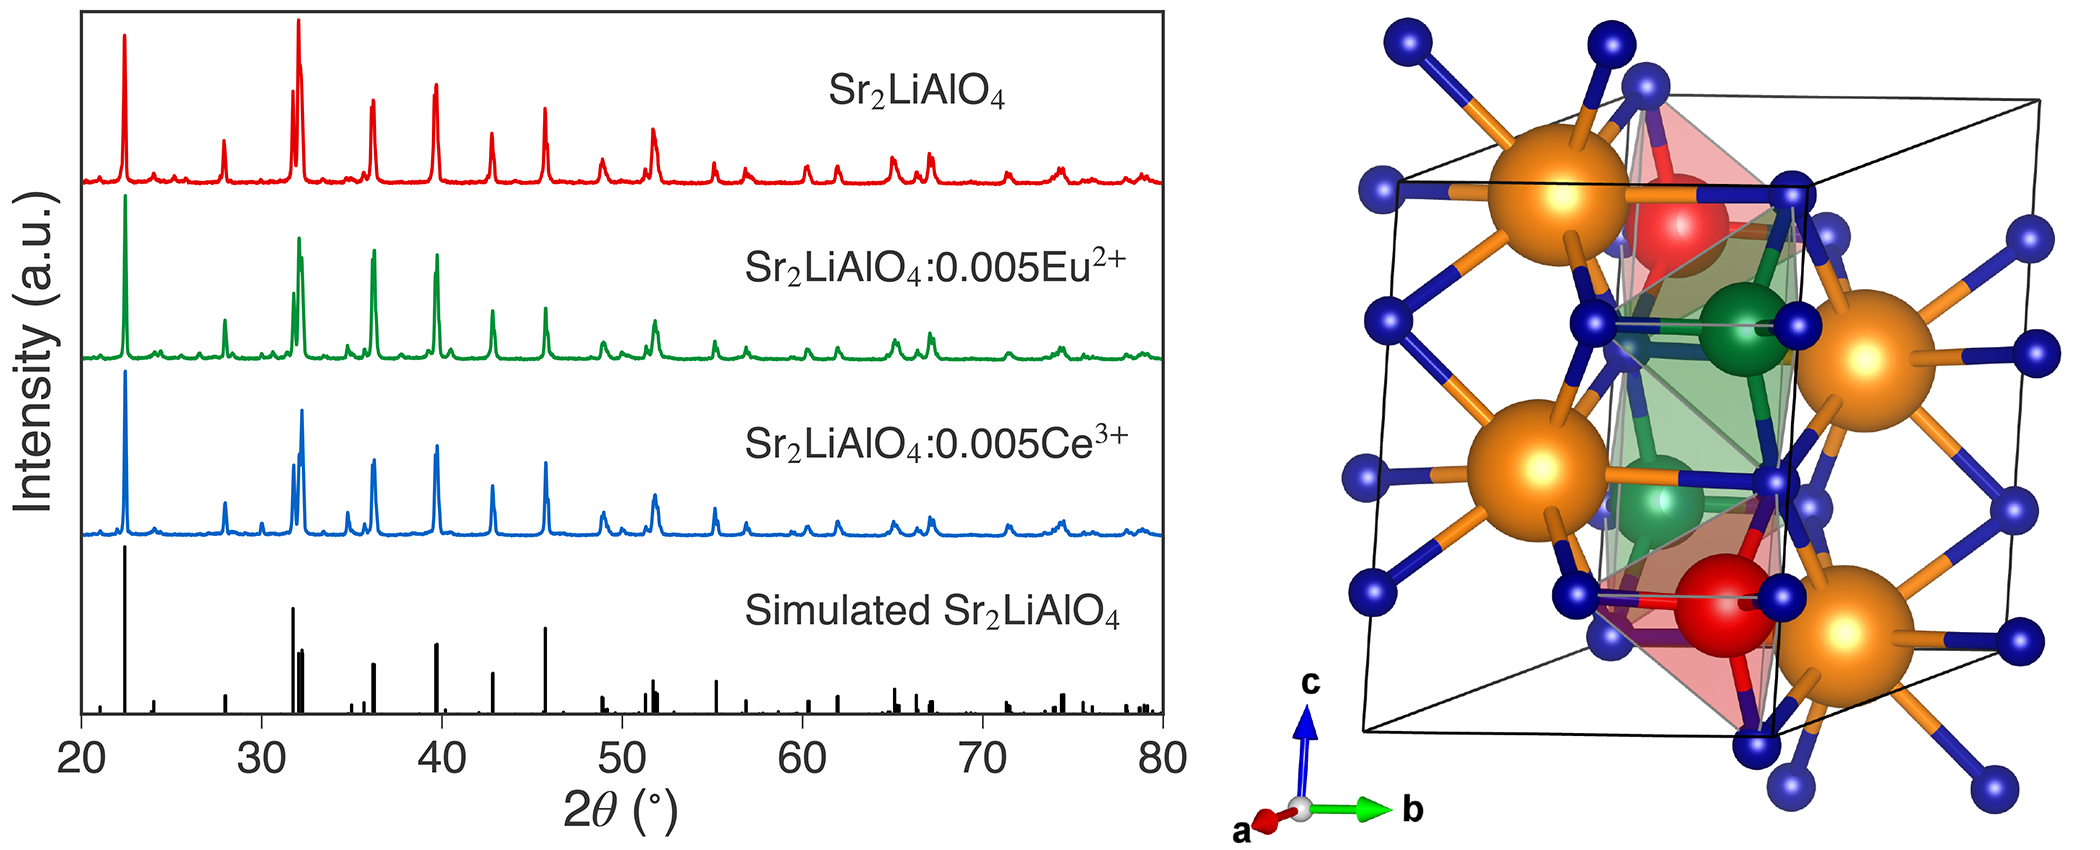
\includegraphics[width=0.6\textwidth]{figures/xrd_pattern.png}
\end{figure}
    \begin{itemize}
        \item Computing the XRD pattern given a crystal structure is easy.
        \item Inverse problem of predicting crystal structure given an XRD pattern is \textbf{very hard} - phase identification is usually done by matching to database of patterns of \textit{known} crystals using Rietveld refinement (see earlier lecture).
        \item Question: Can we use ML to directly predict crystal structure from a given XRD pattern?
    \end{itemize}
\end{frame}


\begin{frame}{Is it doable?}
\begin{figure}
    \centering
    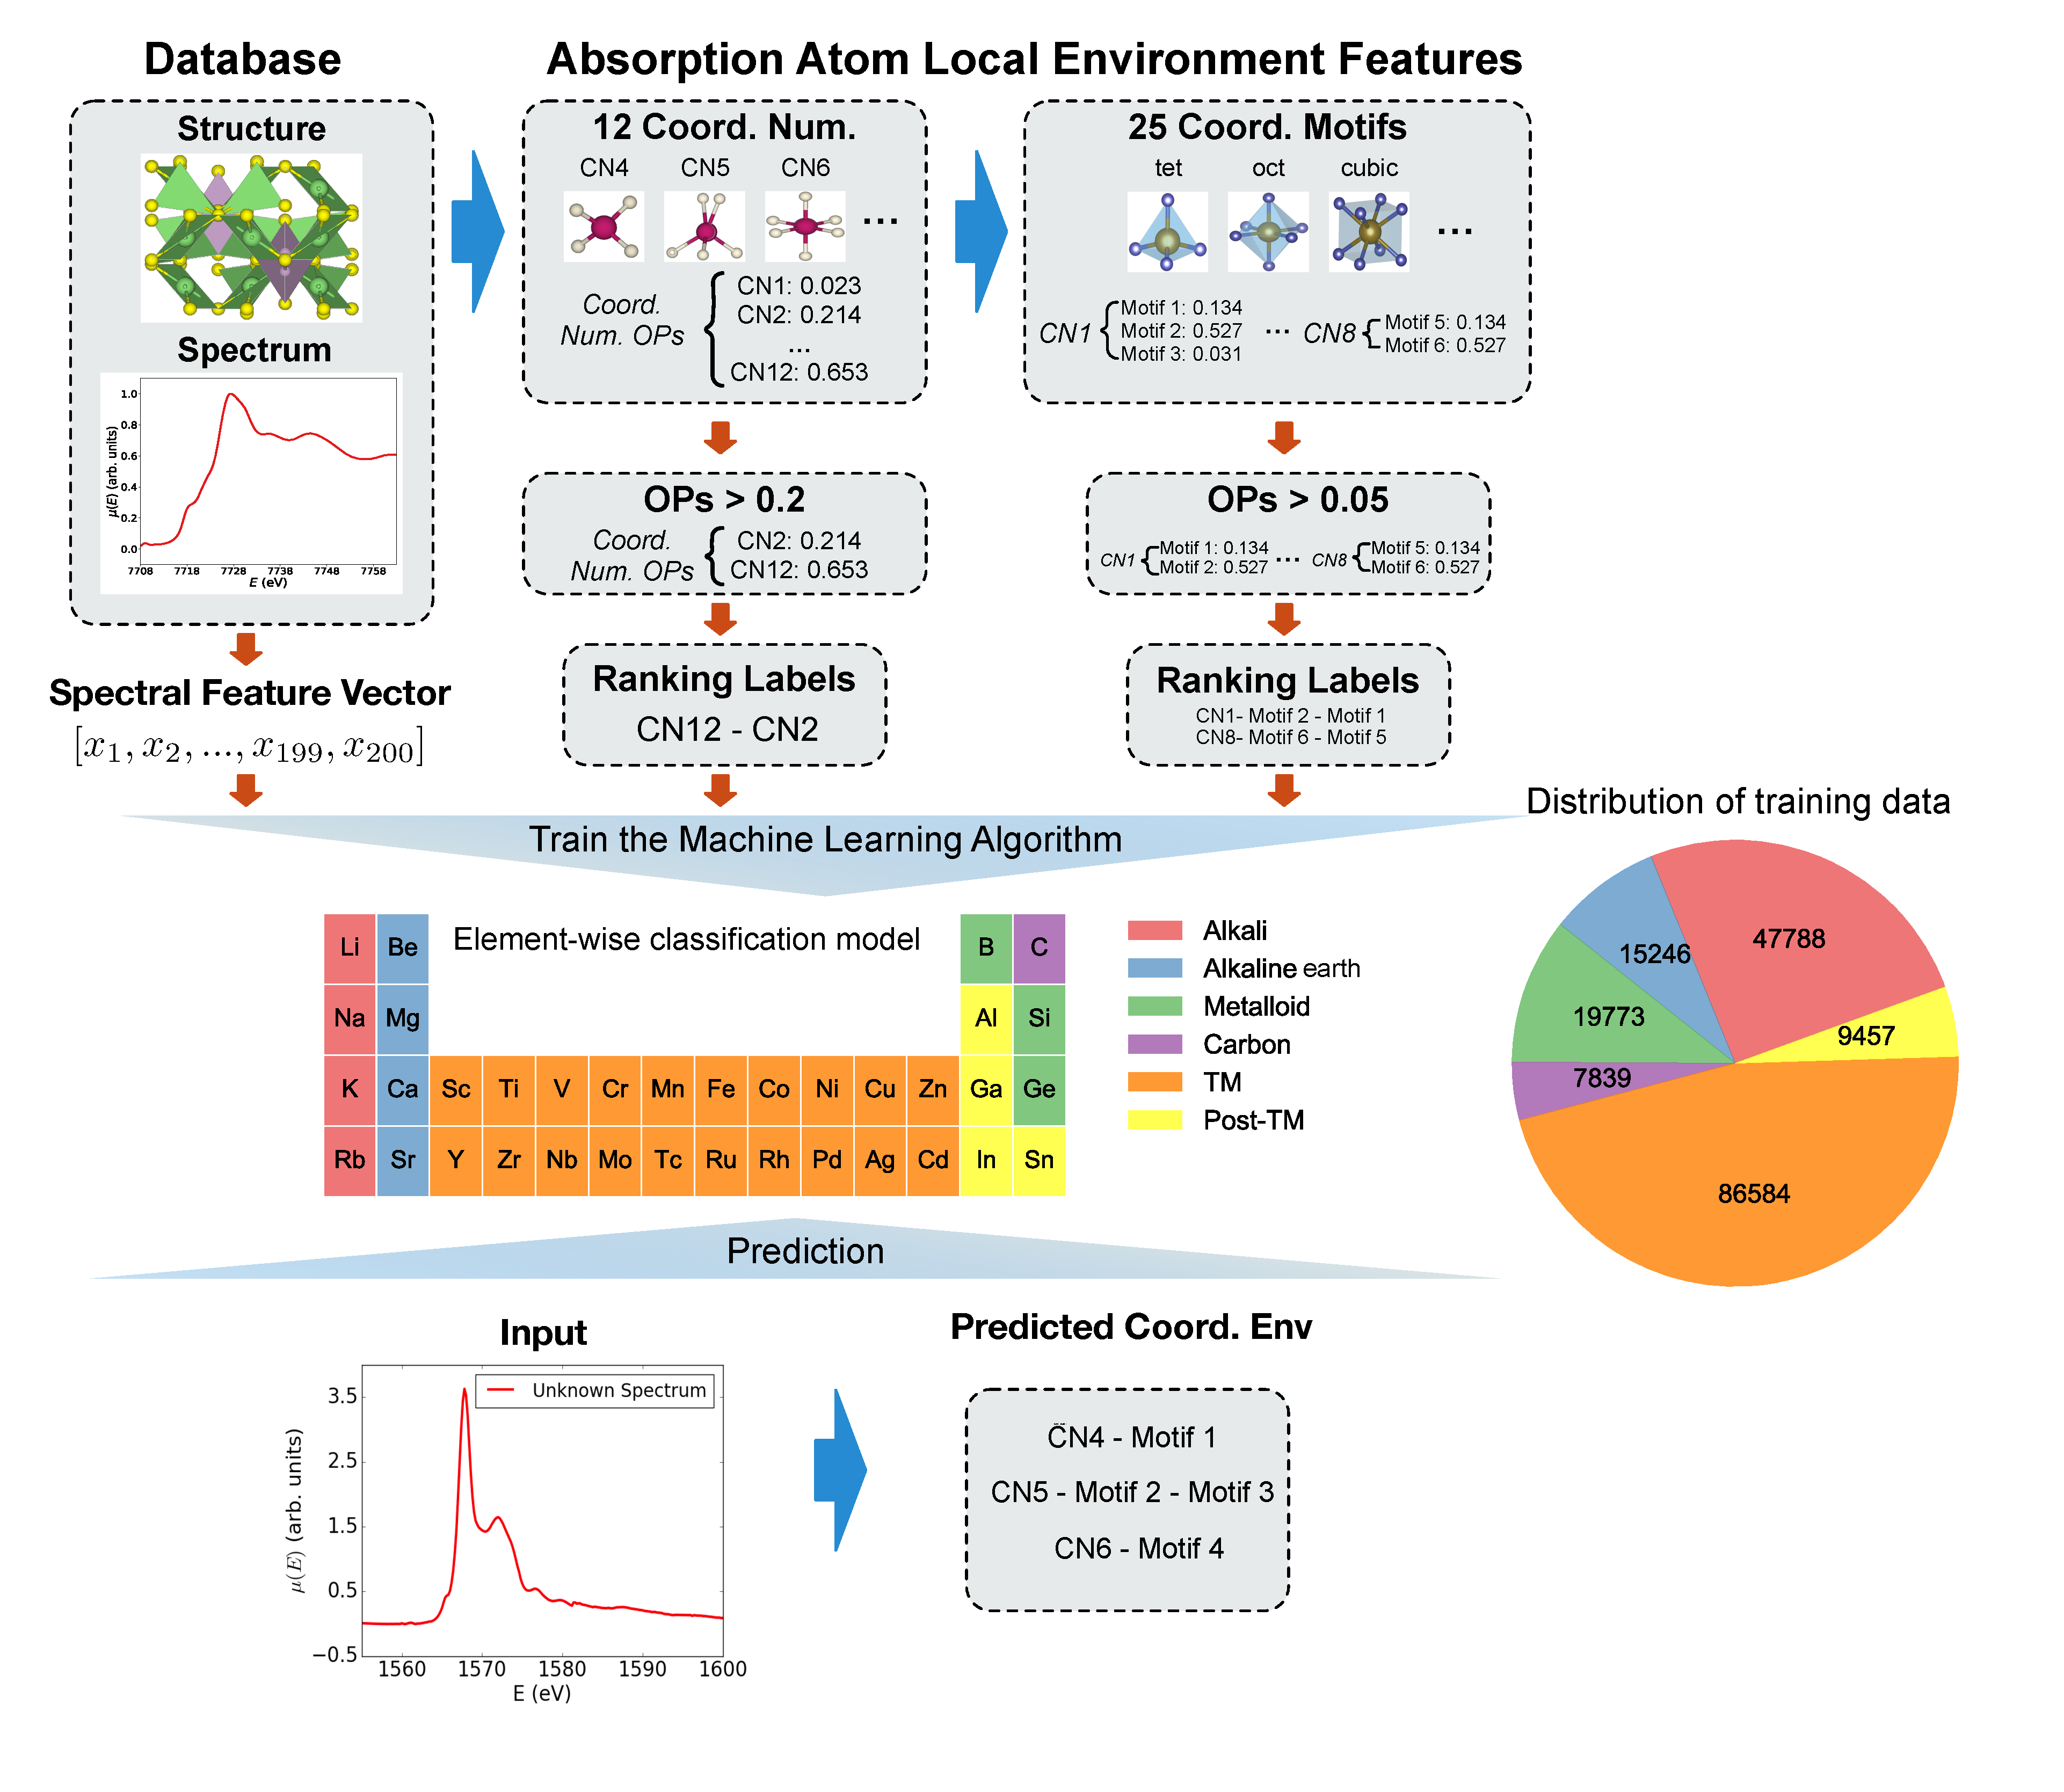
\includegraphics[width=0.4\textwidth]{figures/randomforestxanes.pdf}
    \caption{Workflow for classification of K-edge XANES spectra into one of 25 coordination environments.\cite{zhengRandomForestModels2020}}
\end{figure}
\end{frame}


\begin{frame}{Is it doable, contd?}
\begin{figure}
    \centering
    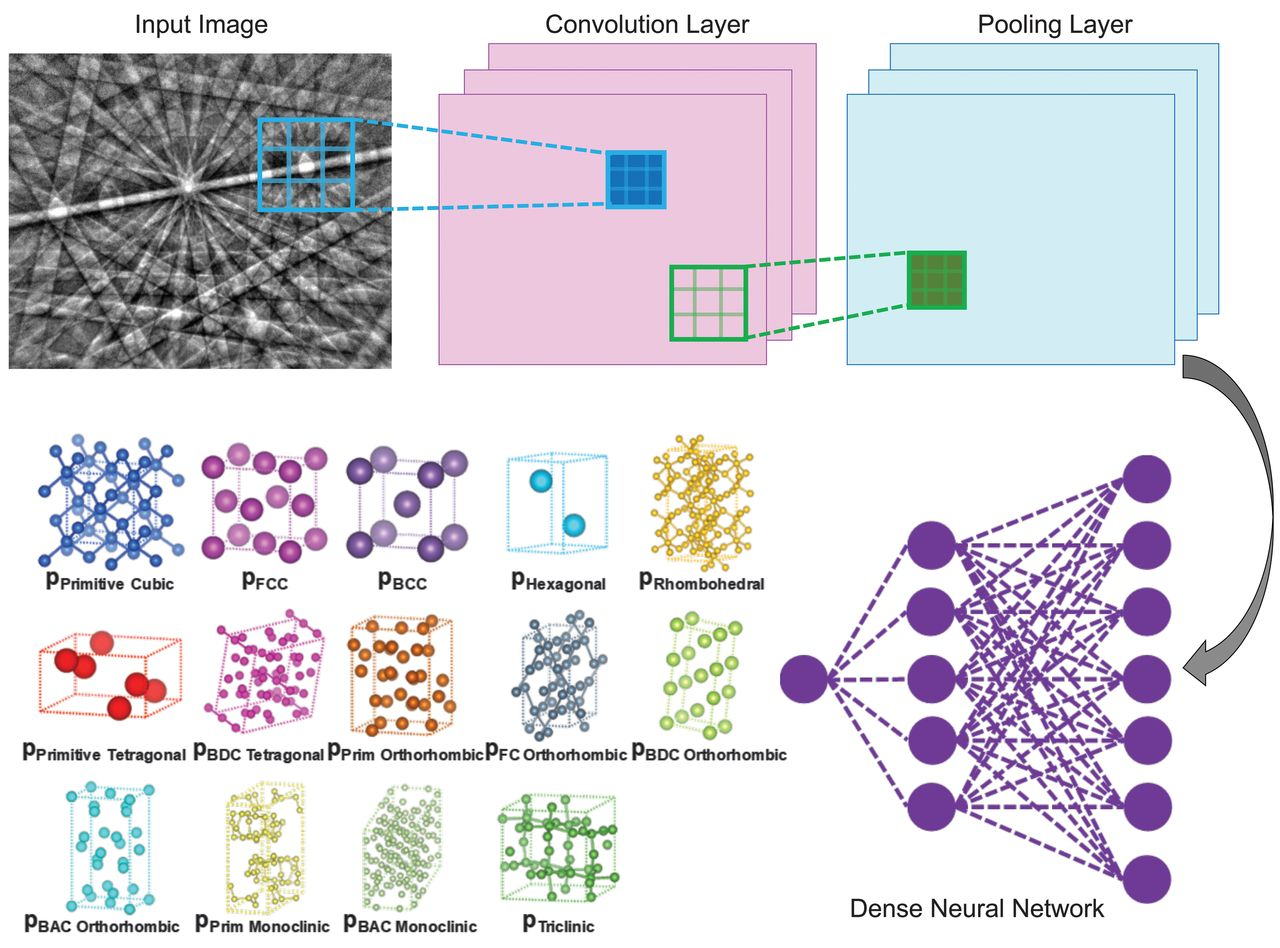
\includegraphics[width=0.5\textwidth]{figures/science-cnn-electron-diffraction.jpg}
    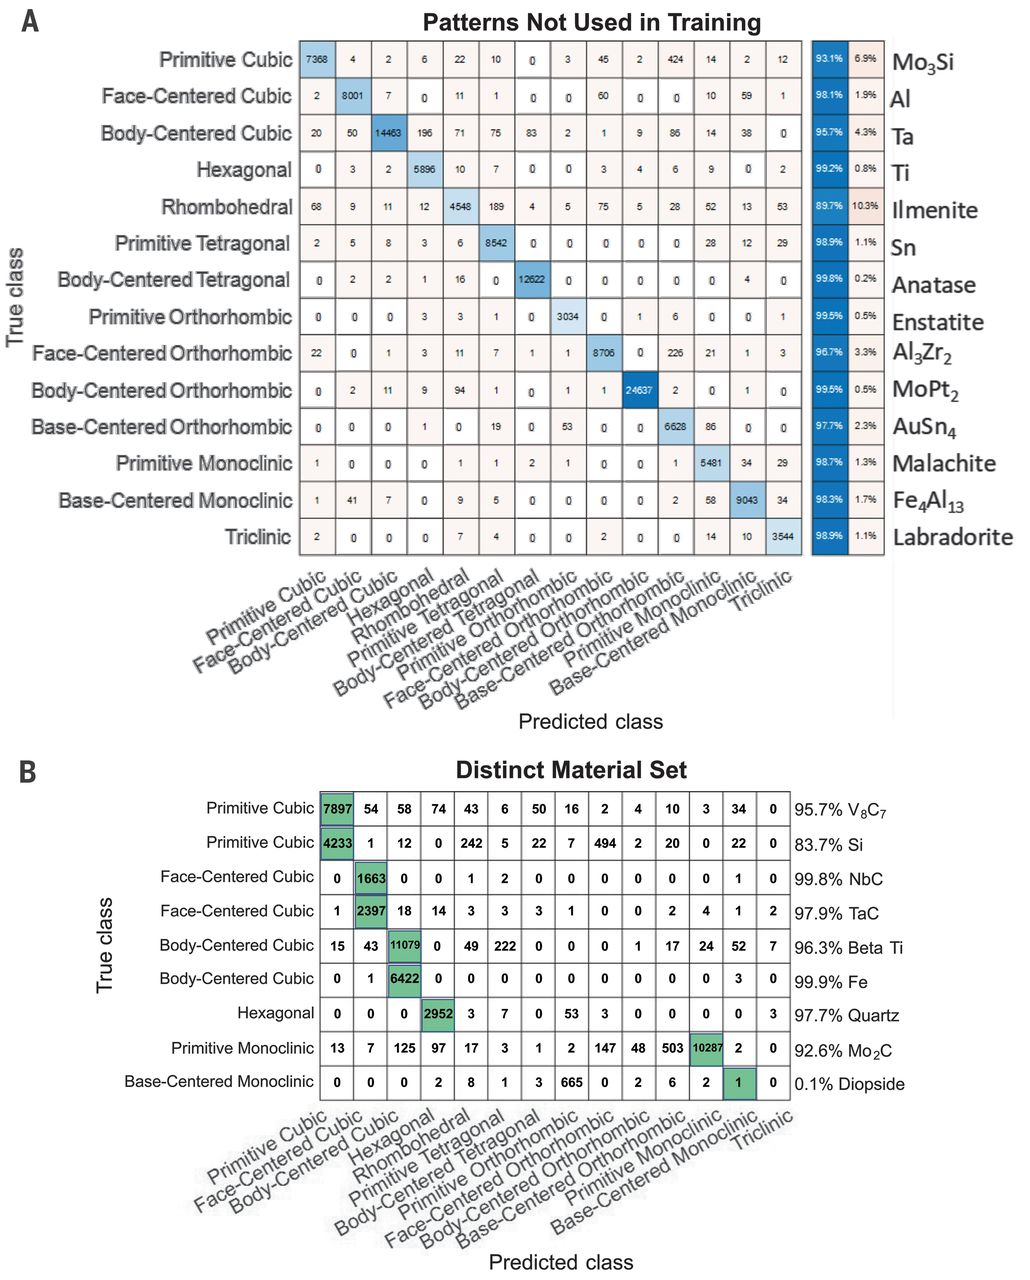
\includegraphics[width=0.3\textwidth]{figures/science-cnn-electron-diffraction2.jpg}
    \caption{CNNs to determine crystal symmetry from electron diffraction patterns with $>$ 90\% accuracy.\cite{kaufmannCrystalSymmetryDetermination2020}}
\end{figure}
\end{frame}


\begin{frame}{The 14 3D Bravais lattices}
\begin{figure}
    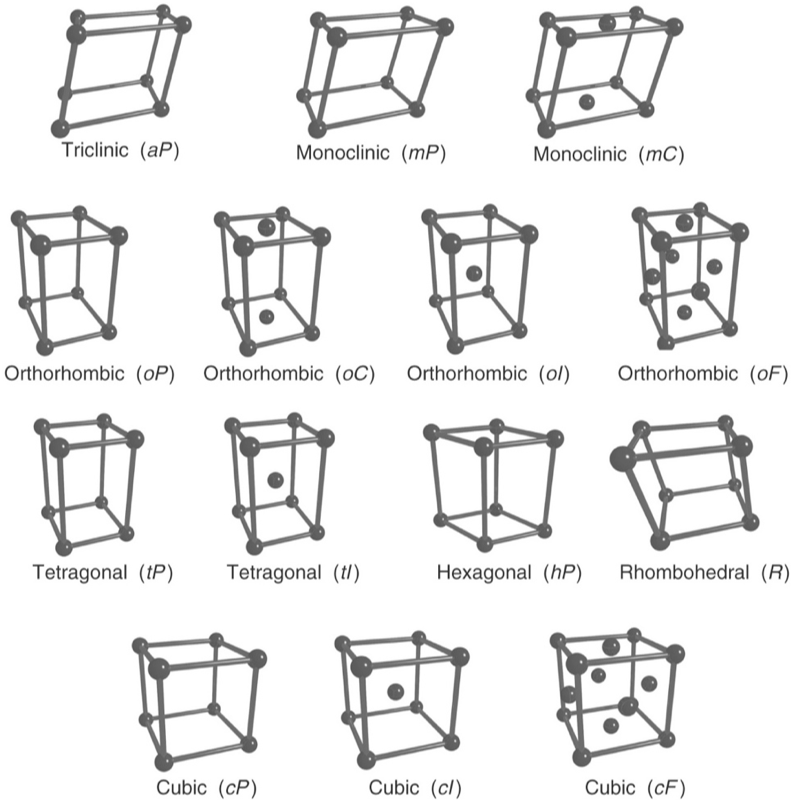
\includegraphics[width=0.4\textwidth]{figures/bravais_lattices.png}
\end{figure}
\end{frame}


\begin{frame}{Dataset}
    \begin{itemize}
        \item $\sim$ 42,000 crystals from Crystallography Open Database
        \item We have already sampled the crystals in a way to somewhat equalize the number of crystals in each Bravais lattice type (note that the actual distribution in the literature is highly biased towards certain lattices).  
    \end{itemize}
    \begin{figure}
        \centering
        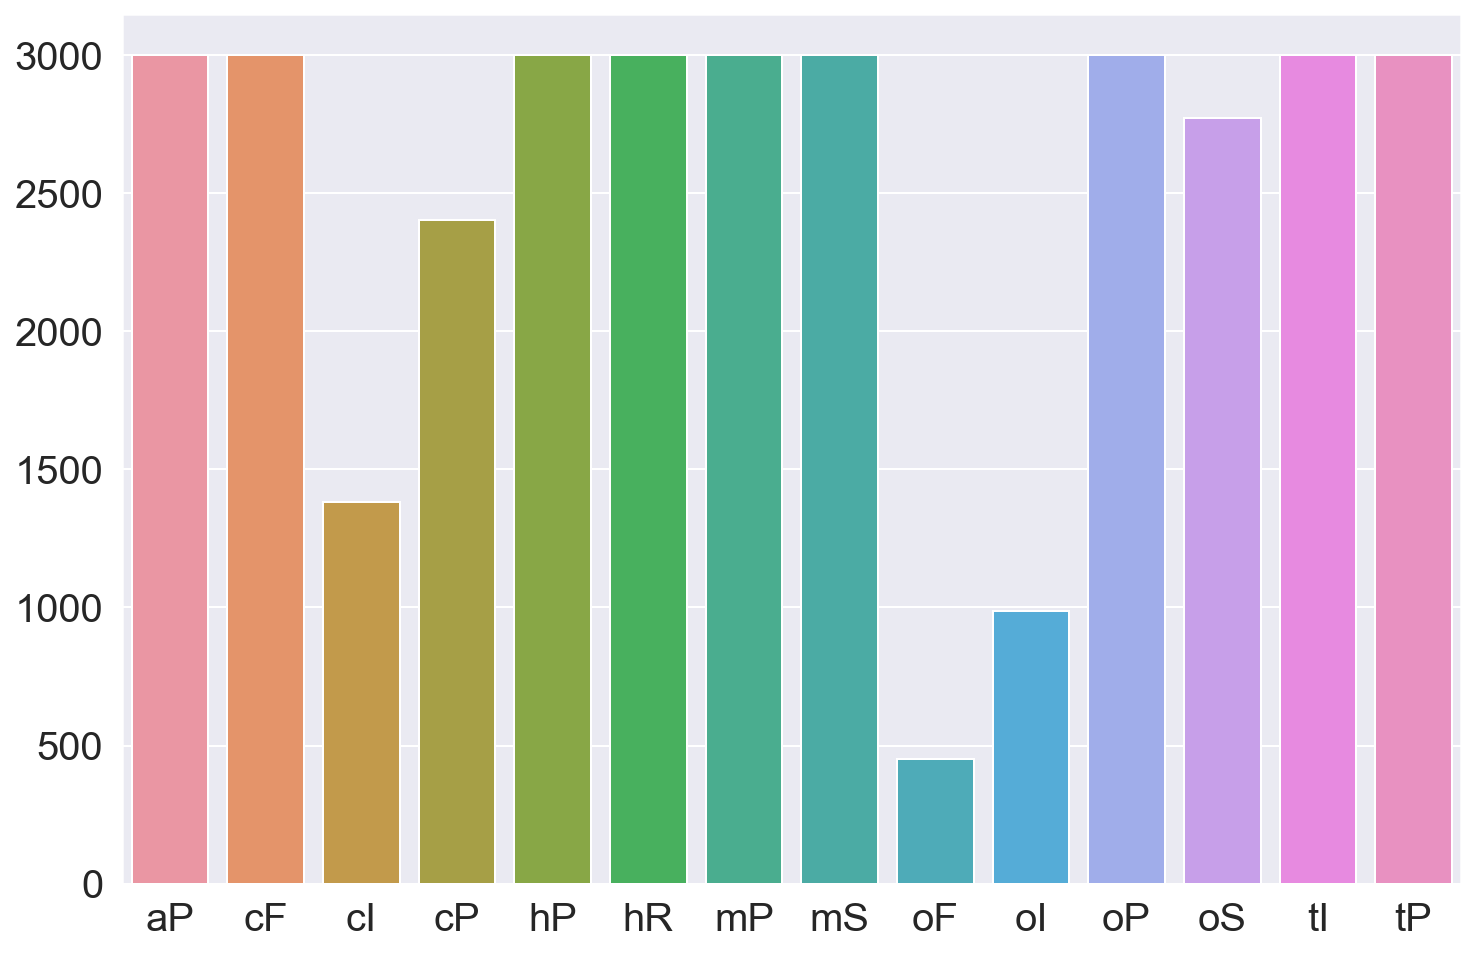
\includegraphics[width=0.45\textwidth]{figures/lab3_data_distribution.png}
    \end{figure}
\end{frame}


\begin{frame}{Dataset, contd.}
\begin{figure}
    \centering
    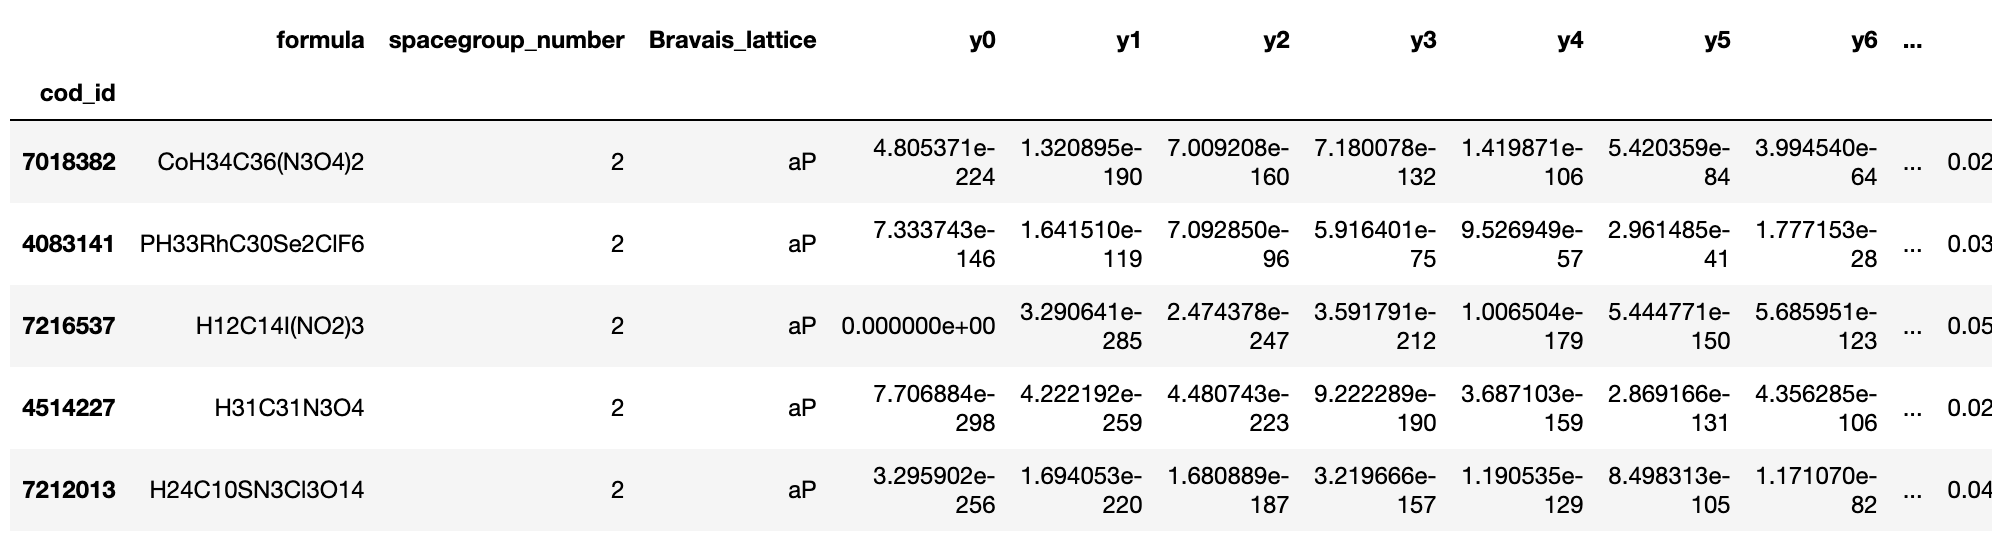
\includegraphics[width=\textwidth]{figures/cod_csv_fmt.png}
\end{figure}
\end{frame}


\begin{frame}{Task}
    \begin{itemize}
        \item Develop a ML model to classify an XRD pattern into one of the 14 Bravais lattices. 
        \item Experiment with any of the ML models that you have learnt, and play around with various parameters. 
        \item \textbf{Hint:} use smaller sample of 10,000 data points to experiment with different models first, before using full data set to do serious model building and optimization. 
        \item Show all parameter optimizations carried out, e.g., grid search. Demonstrate the usage of at least two types of ML model. 
        \item Submission should be done in two places:
        \begin{itemize}
            \item Kaggle, which will have a leaderboard.
            \item Google classroom, where you will submit your Jupyter notebooks.
        \end{itemize}
        \item Discuss the results you have obtained, offering interpretations of how your model is achieving the performance claimed. Compare the results you have obtained with what would have been achieved based on random guessing. Is the ML model doing anything useful?
    \end{itemize}
\end{frame}


\begin{frame}{Evaluation Criteria}
    \begin{itemize}
        \item Grading will be done on the basis of the proper use of data science techniques, e.g., separation of training and test data, validation, parameter search and optimization, coding style and materials science insights. Raw accuracy is not the goal for grading.
        \item Competition evaluation will be based on robust performance achieved.
    \end{itemize}
\end{frame}


\begin{frame}{Next steps}
    \begin{itemize}
        \item Sign up for Kaggle account.
        \item Download the dataset.
        \item Start building your models.
        \item Submission: Please submit at least one model 
    \end{itemize}
\end{frame}


\begin{frame}{Optional challenge problem}
    \begin{itemize}
        \item Instead of classification into 14 Bravais lattices, can an ML algorithm classify an XRD pattern into one of 230 space groups?
    \end{itemize}
\end{frame}


\begin{frame}{Bibliography}
    \bibliographystyle{unsrt}
    \bibliography{refs}
\end{frame}


\begin{frame}
    \Huge{\centerline{The End}}
\end{frame}

\end{document}

